\section{高阶矩上界}
\label{sec:tail-higher-moments}

Chebyshev不等式用平方给远处的质量加权。若把平方换成四次方、六次方，远处的质量在期望里被放得更大，同样大小的矩就迫使远处的质量更少。代价也很明显：要知道更高阶的矩，并且它要有限。

\paragraph{一般的矩上界}
设$a$是任意给定的中心，不必是均值。对非负变量$\lvert X-a\rvert$和$p>0$，函数$s\mapsto s^p$在$[0,\infty)$上严格增，所以对$t>0$，“偏离至少$t$”与“偏离的$p$次方至少$t^p$”是同一个事件。

\begin{theorem}[矩上界]
\label{thm:tail-moment}
设$p>0$，$a\in\mathbb{R}$，且$\mathbb{E}\lvert X-a\rvert^p<\infty$。则对每个$t>0$，
\begin{equation}
 \mathbb{P}(\lvert X-a\rvert\geq t)\leq\frac{\mathbb{E}\lvert X-a\rvert^p}{t^p} .
 \label{eq:tail-moment}
\end{equation}
\end{theorem}

\begin{proof}
因为$t>0$，$p>0$，幂函数$s\mapsto s^p$在$[0,\infty)$上严格增，所以$\lvert X-a\rvert\geq t$当且仅当$\lvert X-a\rvert^p\geq t^p$。$\lvert X-a\rvert^p$非负，期望有限，对它在阈值$t^p>0$处用定理~\ref{thm:tail-markov}：
\[
 \mathbb{P}(\lvert X-a\rvert\geq t)=\mathbb{P}\bigl(\lvert X-a\rvert^p\geq t^p\bigr)\leq\frac{\mathbb{E}\lvert X-a\rvert^p}{t^p} .
\]
这就是式~\eqref{eq:tail-moment}。
\end{proof}

式~\eqref{eq:tail-moment}称为\term{矩上界}（moment bound）。$p=2$、$a=\mu$时它就是Chebyshev不等式；$p=1$时它用的是平均绝对偏离；$p$也可以取非整数，例如$0<p<1$，这在均值都不存在时仍然可用。界按$t^{-p}$衰减，阶数越高，远处衰减越快。

\paragraph{存在条件随阶数加强}
由第~\ref{chap:random-variable-moments}章，$0<p<q$时，$q$阶绝对矩有限蕴含$p$阶绝对矩有限，反之不然。所以使用更高阶的矩是在假设更多。Pareto分布把这一点表现得很清楚：$\alpha=3$时，由第~\ref{sec:tail-events}节的计算，
\[
 \mathbb{E}[X^p]=\frac{3}{3-p},\qquad 0<p<3 ,
\]
$p\geq3$时为$+\infty$。阶数趋于$3$时矩本身趋于无穷，界$3/((3-p)t^p)$的系数随之变大。同样，自由度为$\nu$的t分布只有$p<\nu$阶的绝对矩有限。

\paragraph{贯穿例子的四阶与六阶矩}
对$X\sim\operatorname{Bin}(20,1/2)$，取中心$a=10$。由对称性，$p$阶中心绝对矩是
\[
 m_p=\mathbb{E}\lvert X-10\rvert^p=\frac{2}{2^{20}}\sum_{j=1}^{10}\binom{20}{10+j}j^p .
\]
用表~\ref{tab:tail-binomial}逐项相乘。$p=2$时十项之和是$2621440$，于是$m_2=5$，与方差一致。$p=4$时十项依次为
\[
 \begin{gathered}
 167960,\ 2015520,\ 6279120,\ 9922560,\ 9690000,\\
 6279120,\ 2737140,\ 778240,\ 131220,\ 10000,
 \end{gathered}
\]
和为$38010880$。$p=6$时同样相加，和为$887357440$。乘以$2/2^{20}$，得到
\[
 m_2=5,\qquad m_4=72.5,\qquad m_6=1692.5 .
\]

在$t=5$处比较三个界：
\[
 \frac{m_2}{5^2}=0.2,\qquad \frac{m_4}{5^4}=0.116,\qquad \frac{m_6}{5^6}\approx0.108 .
\]
阶数越高越接近精确值$0.0414$。但在$t=3$处情况相反：
\[
 \frac{m_2}{3^2}\approx0.556,\qquad \frac{m_4}{3^4}\approx0.895,\qquad \frac{m_6}{3^6}\approx2.32 .
\]
六阶的界大于$1$，毫无用处，二阶的界反而最好。

\paragraph{高阶不一定更紧}
原因在于矩把\emph{所有}偏离都按$p$次方加权。偏离小于$t$的质量在$\lvert x-a\rvert^p/t^p$中被压小，偏离大于$t$的质量被放大。$t$较小时，大量质量的偏离与$t$相当或更大，高阶矩被它们放大得很厉害；$t$较大时，远处的质量很少，高阶矩被放大的部分有限，而$t^p$增长得更快。

两个界的交点可以直接解出。四阶界小于二阶界，当且仅当$m_4/t^4<m_2/t^2$，即
\[
 t^2>\frac{m_4}{m_2}=\frac{72.5}{5}=14.5,\qquad t>3.81 .
\]
同理，六阶界小于四阶界当且仅当$t^2>m_6/m_4\approx23.3$，即$t>4.83$。图~\ref{fig:tail-binomial-moment-bounds}显示了这种依次接替：每一阶的界在某个阈值以后才成为最好的。

\begin{BookInlineFigure}
 \centering
 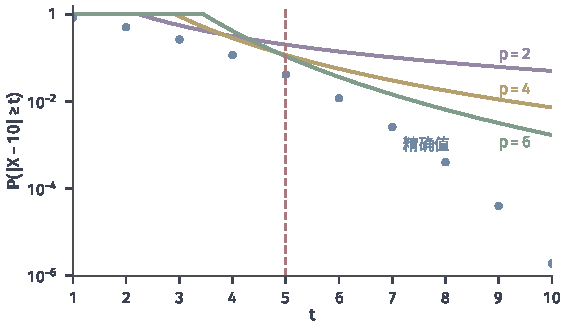
\includegraphics[width=96mm]{figures/07-probability/01-elementary-probability/matplotlib/tail-binomial-moment-bounds/figure.pdf}
 \caption{$X\sim\operatorname{Bin}(20,1/2)$的双侧尾概率$\mathbb{P}(\lvert X-10\rvert\geq t)$（蓝点）与矩上界$\min\{1,m_p/t^p\}$：紫线$p=2$，黄线$p=4$，绿线$p=6$。纵轴为对数刻度，红色虚线标出$t=5$。}
 \label{fig:tail-binomial-moment-bounds}
\end{BookInlineFigure}

\paragraph{给定阈值时选择阶数}
既然没有一个阶数处处最好，自然的做法是对给定的$t$，在所有可用的阶数中取最小的界。标准高斯分布的各阶矩都有限，可以把这件事算到底。记$\varphi(x)=\mathrm{e}^{-x^2/2}/\sqrt{2\pi}$，它满足$\varphi'(x)=-x\varphi(x)$。对$p\geq0$分部积分，边界项因$\varphi$衰减极快而为零，得到
\[
 \mathbb{E}[Z^{p+2}]=\int_{-\infty}^{\infty}x^{p+1}\cdot x\varphi(x)\,\mathrm{d}x=(p+1)\int_{-\infty}^{\infty}x^{p}\varphi(x)\,\mathrm{d}x=(p+1)\,\mathbb{E}[Z^p] .
\]
从$\mathbb{E}[Z^0]=1$出发，偶数阶矩为
\[
 \mathbb{E}[Z^{p}]=(p-1)(p-3)\cdots3\cdot1,\qquad p=2,4,6,\dots .
\]因此从$p$阶换到$p+2$阶，界乘上因子
\[
 \frac{\mathbb{E}[Z^{p+2}]/t^{p+2}}{\mathbb{E}[Z^p]/t^p}=\frac{p+1}{t^2} .
\]
只要$p+1<t^2$，提高阶数就让界变小；一旦$p+1>t^2$，再提高就变大。

$t=2$时$t^2=4$，从$p=2$到$p=4$乘$3/4$，再到$p=6$乘$5/4$，所以最好的偶数阶是$p=4$，界为$3/16=0.1875$。$t=3$时$t^2=9$，从$p=6$到$p=8$乘$7/9$，从$p=8$到$p=10$乘$9/9=1$，界在$p=8$和$p=10$处同为
\[
 \frac{\mathbb{E}[Z^8]}{3^8}=\frac{105}{6561}\approx0.0160 .
\]
奇数阶的绝对矩也可以计算，$p=9$时略小，约为$0.0156$；精确值是$2Q(3)\approx0.0027$。

图~\ref{fig:tail-normal-moment-order}把界作为阶数的函数画出来：曲线先降后升，最低点随$t$右移。最优阶数大约是$t^2$，阈值越远，越要用高阶矩。若只允许用某个固定阶数$p$，界只能按$t^{-p}$衰减，而高斯尾部比任何幂次都衰减得快。要跟上这种衰减，就需要把各阶矩一起利用，这正是下一节指数矩的作用。

\begin{BookInlineFigure}
 \centering
 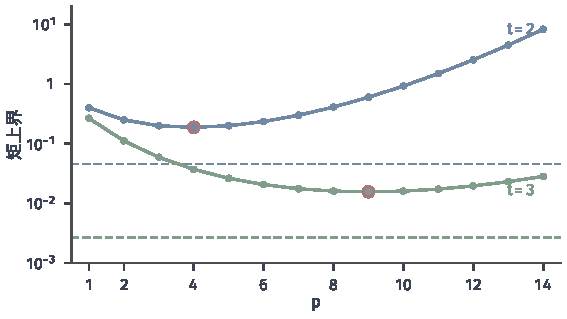
\includegraphics[width=96mm]{figures/07-probability/01-elementary-probability/matplotlib/tail-normal-moment-order/figure.pdf}
 \caption{$Z\sim\mathcal{N}(0,1)$的矩上界$\mathbb{E}\lvert Z\rvert^p/t^p$随阶数$p$的变化，纵轴为对数刻度。蓝色为$t=2$，绿色为$t=3$，红圈是整数阶中的最小值，同色虚线是精确值$\mathbb{P}(\lvert Z\rvert\geq t)$。}
 \label{fig:tail-normal-moment-order}
\end{BookInlineFigure}
